\section{DATABASE STRUCTURE DESIGN}
\label{section:design}

\subsection{Specification of the dataset}
\label{sect:sub-title}
Identify the relevant entities, attributes, and relationships together with any 
constraints and properties

\subsection{E-R Diagram}
\label{sect:sub-title}
The ER-Diagram(Fig.1) of our system contains four entities
and two relations.
\begin{figure}[H]
    \centering
    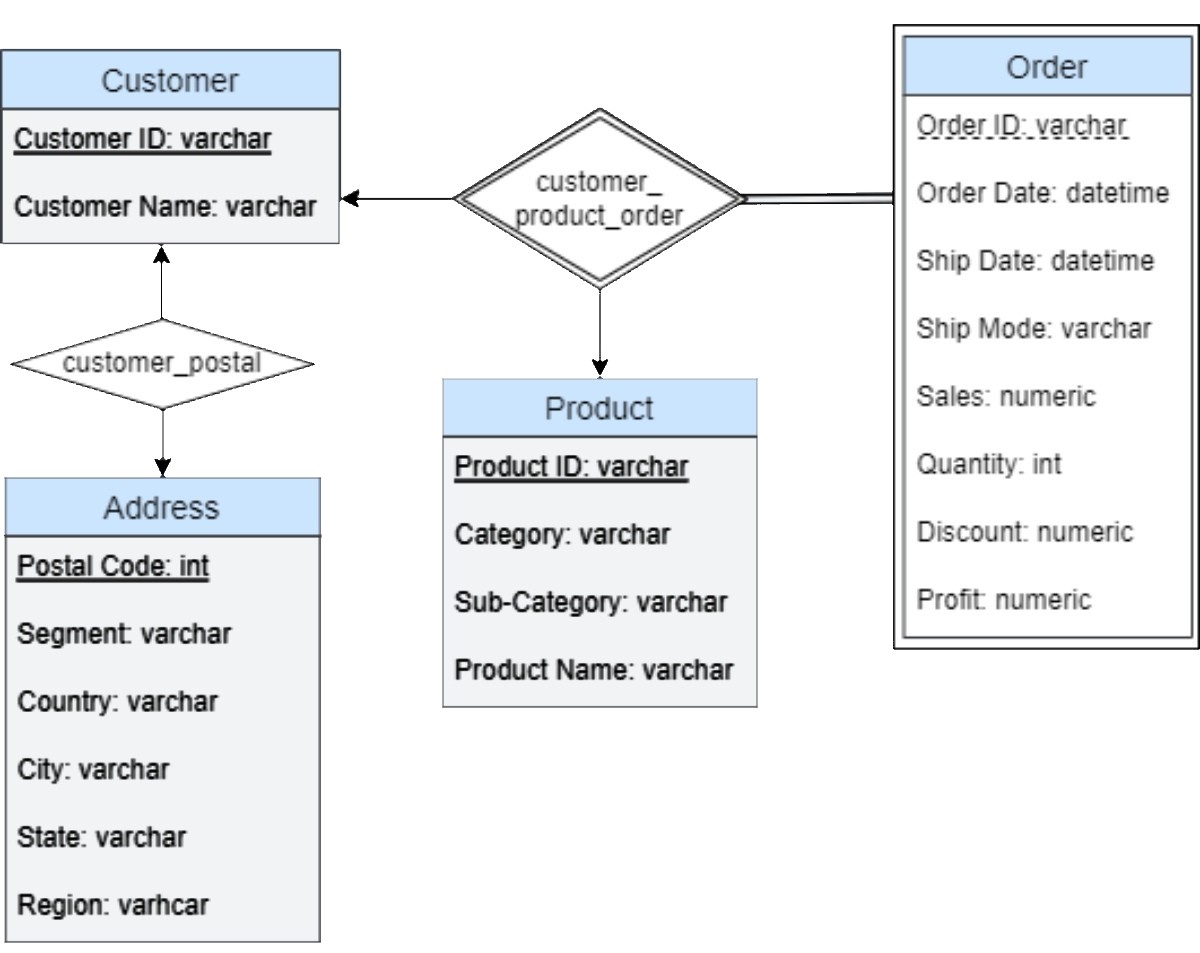
\includegraphics[width=\columnwidth]{images/ER.jpg}
    \caption[Short text]{ER Diagram of Supermarket Management System.}
    \label{fig:ER}
\end{figure}


\subsection{relational schema}
\label{sect:sub-title}
Convert the E-R diagrams to relational schema (clearly indicating the primary
keys, foreign keys, functional and/or multi-valued dependencies\newline
Customer \{\underline{CustomerID}, Customer\_Name\} \newline
Product \{\underline{ProductID}, Category, Sub\_Category, Product\_Name\} \newline
Order \{\underline{Order\_ID}, \underline{CustomerID}, \underline{ProductID}, Order\_Date, Ship\_Date, Ship\_Mode, Sales, Quantity, Discount, Profit\}\newline
Address \{\underline{Postal\_Code}, segment,  Country, City, State,  Region\}\newline
customer\_product\_order \{CustomerID, ProductID, Order\_ID \}\newline
customer\_postal \{CustomerID, Postal\_Code\}

\subsection{Normalization of Schema}
\label{sect:sub-title}
Schema \& Normalization

\subsection{Index and Hashing}
\label{sect:sub-title}
Index \& Hashing